\begin{figure}[ht]
    \centering
    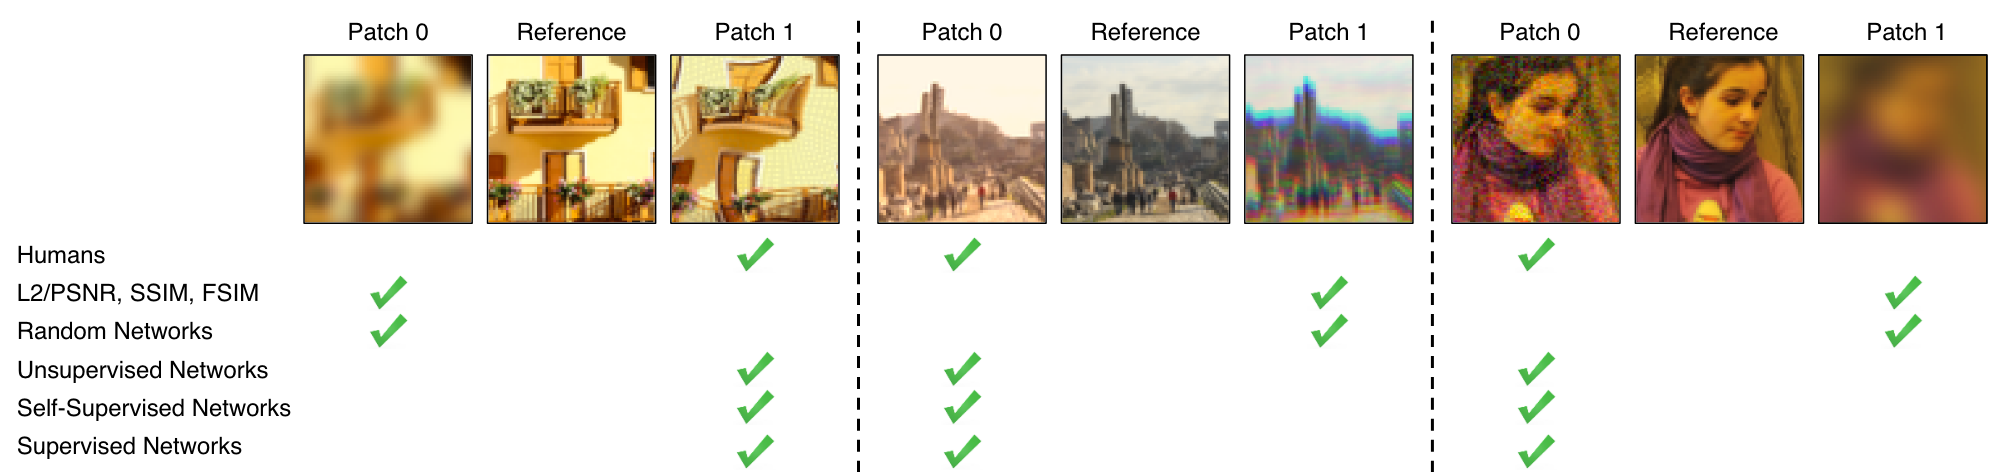
\includegraphics[width=1.0\textwidth]{figures/lpips.png}
    \caption[LPIPS - Learned Perceptual Image Patch Similarity]{\acrshort{lpips} is trained to perceive image similarity the same way humans do. The dataset used to train the similarity metric contains two types of perceptual judgements, \acrshort{2afc} and \acrshort{jnd}. With \acrshort{2afc} people were asked to select which of the distorted images was "closer" to the reference. With \acrshort{jnd} people were presented with 2 image patches, one reference and one distorted, and asked if they were the same. Figure 1 from LPIPS \cite{zhang_unreasonable_2018}.}
    \label{fig:lpips}
\end{figure}

